\chapter{Design og implementering}


\section{Software Design}

\subsection{Klassediagrammer}

\subsubsection{PSoC0}
På figur \ref{figure:PSoC0KlasseDiagram} ses klassediagrammet indeholdende klasserne som bruges af softwaren allokeret på CPU'en PSoC0.

\begin{figure}[H]
	\centering
	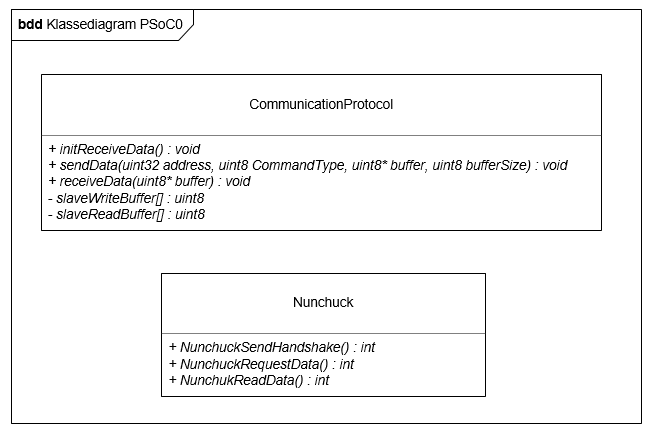
\includegraphics[width=\textwidth]{DesignOgImplementering/images/PSoC0KlasseDiagram}
	\caption{Klassediagram for CPU'en PSoC0}
	\label{figure:PSoC0KlasseDiagram}
\end{figure}

På figur \ref{figure:PSoC0KlasseDiagram} kan det ses at softwaren på PSoC0 CPU'en gør brug af klasserne \textit{CommunicationProtocol} samt \textit{Nunchuck}

\subsection{Afkodning af Wii-Nunchuck Data Bytes}
Aflæste bytes fra Wii-Nunchuck - indeholdende tilstanden af knapperne og det analoge stick - er kodet når de oprindeligt modtages via I2C bussen. Disse bytes skal altså afkodes før deres værdier er brugbare. Afkodningen af hver byte sker ved brug af følgende formel:

\textit{AfkodetByte = (AflæstByte XOR 0x17) + 0x17}

Fra formlen kan det ses at den aflæste byte skal \textit{XOR}'s (Exclusive Or) med værdien 0x17, hvorefter dette resultat skal adderes med værdien 0x17.

\subsection{Kalibrering af Wii-Nunchuck Analog Stick}
De afkodede bytes for Wii-Nunchuck's analoge stick har definerede standardværdier for dets forskellige fysiske positioner. Disse værdier findes i tabel \ref{tabel:WiiNunchuckStickPositioner}

\begin{table}[H]
	\centering
	\begin{tabular}{|l|l|}
		\hline
		X-akse helt til venstre & 0x1E \\ \hline
		X-akse helt til højre   & 0xE1 \\ \hline
		X-akse centreret        & 0x7E \\ \hline
		Y-akse centreret        & 0x7B \\ \hline
		Y-akse helt frem        & 0x1D \\ \hline
		Y-akse helt tilbage     & 0xDF \\ \hline
	\end{tabular}
	\caption{Standardværdier for fysiske positioner af Wii-Nunchuck's analoge stick}
	\label{tabel:WiiNunchuckStickPositioner}
\end{table}

I praksis skal de afkodede værdier for det analoge stick kalibreres, da slør pga. brug gør at de ideale værdier ikke rammes. 

I projektet er de afkodede værdier for det analoge stick kalibreret med værdien -15 (0x0F i hexadecimal), altså ser den endelige formel for afkodning samt kalibrering således ud:

\textit{AfkodetByte = (AflæstByte XOR 0x17) + 0x17 - 0x0F}

\section{Hardware Design}
På baggrund af BDD'et er der fundet følgende hardwareblokke, der skal udarbejdes: 
\begin{itemize}
	\item Motorstyring
	\item Tre motorer
\end{itemize}

\subsection{Motorstyring}
Til at styre de tre motorer er der bygget en H-bro, der skal bruges i tre eksemplarer. To af disse motorer skal kunne styre kanonen, så den kan køre op og ned og frem og tilbage. Den tredje skal bruges til at styre affyringsekanismen. 

\subsubsection{H-bro}
Først blev der designet en H-bro, som bestod af to N-MOSFET's af typen IRLZ44 og to P-MOSFET's af typen ZVP3306. Denne kan ses på figur... Det viste sig dog, at den P-MOSFET der var brugt, var for svag til at kunne trække den strøm, som motoren skulle bruge, hvilket betød, at den blev brændt af. 


\begin{figure}[H]
	\centering
	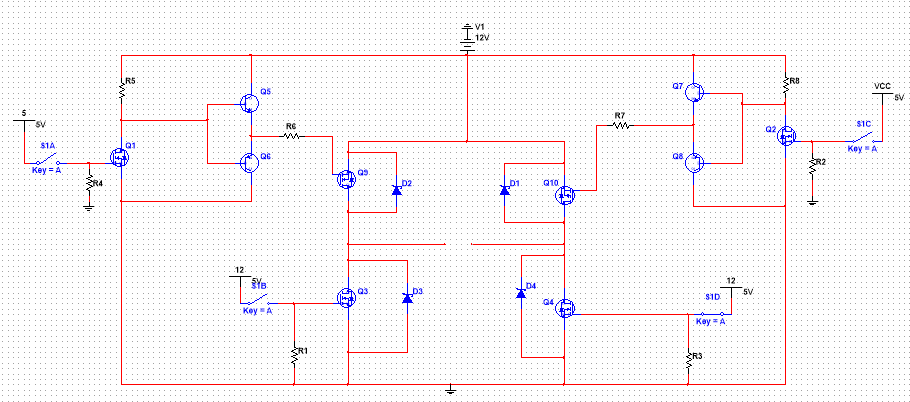
\includegraphics[]{DesignOgImplementering/images/motorkreds}
	\caption{H-bro kredsløb}
	\end{figure}

\begin{table}[]
	\centering
	\caption{Komponentbetegnelser på H-bro}
	\label{my-label}
	\begin{tabular}{|l|l|l}
		\cline{1-2}
		Betegnelse 	& Komponent 	          	 &  \\ \cline{1-2}
		VCC        	& 5V                         &  \\ \cline{1-2}
		Q1   		& IRLZ44(mosfet N-Channel)   &  \\ \cline{1-2}
		Q2   		& IRLZ44(mosfet N-Channel)   &  \\ \cline{1-2}
		Q3   		& IRLZ44(mosfet N-Channel)   &  \\ \cline{1-2}
		Q4   		& IRLZ44(mosfet N-Channel)   &  \\ \cline{1-2}
		Q5   		& BC547                      &  \\ \cline{1-2}
		Q6   		& BC557                      &  \\ \cline{1-2}
		Q7   		& BC547                      &  \\ \cline{1-2}
		Q8   		& BC557                      &  \\ \cline{1-2}
		Q9   		& IRF9Z34N(mosfet P-Channel) &  \\ \cline{1-2}
		Q10  		& IRF9Z34N(mosfet P-Channel) &  \\ \cline{1-2}
		R1   		& 10k$\Omega$                &  \\ \cline{1-2}
		R2   		& 10k$\Omega$                &  \\ \cline{1-2}
		R3   		& 10k$\Omega$                &  \\ \cline{1-2}
		R4   		& 10k$\Omega$                &  \\ \cline{1-2}
		R5   		& 10k$\Omega$                &  \\ \cline{1-2}
		R6   		& 100$\Omega$                &  \\ \cline{1-2}
		R7   		& 100$\Omega$                &  \\ \cline{1-2}
		R8   		& 10k$\Omega$                &  \\ \cline{1-2}
		D1   		& IN5819                     &  \\ \cline{1-2}
		D2   		& IN5819                     &  \\ \cline{1-2}
		D3   		& IN5819                     &  \\ \cline{1-2}
		D4   		& IN5819                     &  \\ \cline{1-2}
	\end{tabular}
\end{table}

\subsubsection{Mosfet}
Til at styre motoren er der bygget en H-bro, som består af fire mosfet, hvor to af dem er af typen IRF9Z34N (mosfet P-channel, som er Q9 og Q10 på kredsløbstegningen) og de to andre mosfet er af typen IRLZ44 (mosfet N-Channel, som er Q3 og Q4 kredsløbstegningen). Det er valgt at bruge mosfet for at kunne styre H-broen, da det ved denne er muligt at lukke og åbne for spændingen, og de bliver styret af spænding, i forhold til transistorer, som bliver styret af strøm. 

\begin{itemize}
	\item Mosfet N-channel:\\
	\item 
	Mosfet P-channel: \\
	Den kan klare en strøm på 6,7A ifølge databladet. Det vil altså ikke komme til at påvirke motoren, som kan trække en strøm på 0,35A. 
	
	For at der kan løbe spænding igennem IRF9Z34N(mosfet P-channel), så skal den have en negativ spænding for at åbne og en spænding på over 0V for at lukke. 
	
\end{itemize}
\subsubsection{Diode}
Over fire af mosfetene (Q9, Q10, Q3 og Q4) er der sat en diode af typen IN5819. Den skal fungere som beskyttelse af de fire mosfet (Q9, Q10, Q3 og Q4). Det, de gør, er, at de sikrer, at den spænding, som er tilbage i motoren, når man lukker for mosfetene, ikke løber tilbage ind i mosfetene og brænder dem af.

\subsubsection{Modstande}
\begin{itemize}
	\item Pull down modstande:\\
	Der er blevet brugt fire modstande (R1, R2, R3 og R4), som pull down modstande, som sørger for, at signalet vil blive holdt lavt, når der ikke er trykket, så det ben ikke står og flyver, så det kan komme til at åbne en mosfet, ved fejl og derved kommer til at brænde en mosfet eller motoren af. Der er valgt en modstand på 10kOhm, som er lille nok til at trække de små spændinger ned, når der ikke er trykket og den stor nok til at spændingen ikke løber der ned, når der er trykket.
	\item modstande
	\begin{itemize}
		\item R6 og R7
		
		\item R5 og R8
	\end{itemize}
	
	
\end{itemize}
\subsubsection{Motor}